\documentclass[border=4pt]{standalone}
% Shared typography and colours for the standalone figures.
\usepackage{unicode-math}
\setmainfont{TeX Gyre Termes}
\setsansfont{TeX Gyre Heros}
\setmonofont{TeX Gyre Cursor}
\setmathfont{TeX Gyre Termes Math}
\usepackage{tikz}
\usetikzlibrary{arrows.meta,positioning,calc,decorations.pathreplacing}
\usepackage{pgfplots}
\pgfplotsset{compat=1.18}
\definecolor{elemA}{HTML}{1F5FA8}
\definecolor{elemB}{HTML}{B8461B}
\definecolor{elemC}{HTML}{2E7D32}
\definecolor{elemD}{HTML}{6A4C93}
\definecolor{frameline}{HTML}{555555}

\usepackage[american]{circuitikz}
\begin{document}
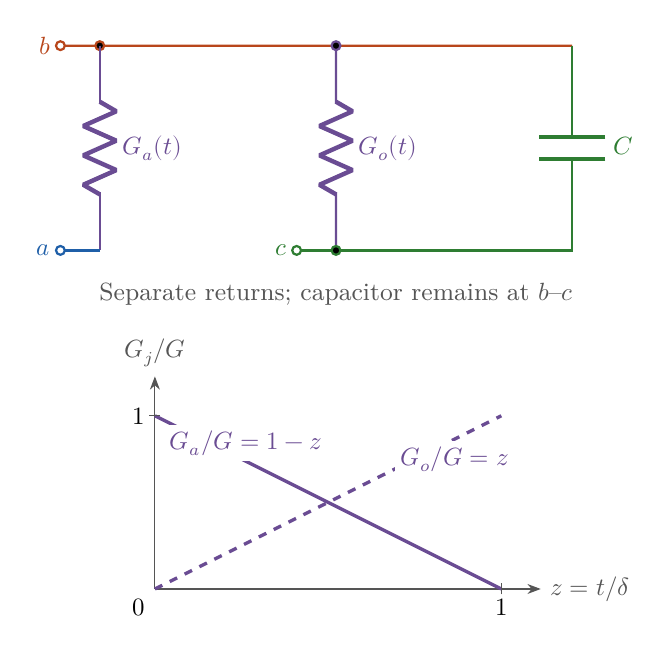
\begin{tikzpicture}[font=\small]
  \draw[elemB,thick] (-0.5,3) node[left] {$b$} to[short,o-*] (0,3)
    -- (3,3) -- (6,3);
  \draw[elemD,thick] (0,3) to[R,l=$G_a(t)$] (0,0.4);
  \draw[elemA,thick] (0,0.4) to[short,-o] (-0.5,0.4) node[left] {$a$};
  \draw[elemD,thick] (3,3) to[R,l=$G_o(t)$,*-] (3,0.4);
  \draw[elemC,thick] (6,3) to[C,l=$C$] (6,0.4)
    -- (3,0.4) to[short,*-o] (2.5,0.4) node[left] {$c$};
  \node[align=center,text=frameline] at (3,-0.15)
    {Separate returns; capacitor remains at $b$--$c$};
  \begin{scope}[shift={(0.7,-3.9)}]
    \draw[-{Stealth},frameline] (0,0) -- (4.9,0) node[right] {$z=t/\delta$};
    \draw[-{Stealth},frameline] (0,0) -- (0,2.7) node[above] {$G_j/G$};
    \draw[elemD,very thick] (0,2.2) -- (4.4,0);
    \draw[elemD,very thick,dashed] (0,0) -- (4.4,2.2);
    \draw[frameline] (-0.07,2.2) -- (0.07,2.2);
    \draw[frameline] (4.4,-0.07) -- (4.4,0.07);
    \node[left] at (0,2.2) {$1$};
    \node[below left] at (0,0) {$0$};
    \node[below] at (4.4,0) {$1$};
    \node[fill=white,inner sep=2pt,text=elemD] at (1.15,1.85) {$G_a/G=1-z$};
    \node[fill=white,inner sep=2pt,text=elemD] at (3.8,1.65) {$G_o/G=z$};
  \end{scope}
\end{tikzpicture}
\end{document}
